% Options for packages loaded elsewhere
\PassOptionsToPackage{unicode}{hyperref}
\PassOptionsToPackage{hyphens}{url}
%
\documentclass[
]{article}
\usepackage{amsmath,amssymb}
\usepackage{lmodern}
\usepackage{iftex}
\ifPDFTeX
  \usepackage[T1]{fontenc}
  \usepackage[utf8]{inputenc}
  \usepackage{textcomp} % provide euro and other symbols
\else % if luatex or xetex
  \usepackage{unicode-math}
  \defaultfontfeatures{Scale=MatchLowercase}
  \defaultfontfeatures[\rmfamily]{Ligatures=TeX,Scale=1}
\fi
% Use upquote if available, for straight quotes in verbatim environments
\IfFileExists{upquote.sty}{\usepackage{upquote}}{}
\IfFileExists{microtype.sty}{% use microtype if available
  \usepackage[]{microtype}
  \UseMicrotypeSet[protrusion]{basicmath} % disable protrusion for tt fonts
}{}
\makeatletter
\@ifundefined{KOMAClassName}{% if non-KOMA class
  \IfFileExists{parskip.sty}{%
    \usepackage{parskip}
  }{% else
    \setlength{\parindent}{0pt}
    \setlength{\parskip}{6pt plus 2pt minus 1pt}}
}{% if KOMA class
  \KOMAoptions{parskip=half}}
\makeatother
\usepackage{xcolor}
\usepackage[margin=1in]{geometry}
\usepackage{color}
\usepackage{fancyvrb}
\newcommand{\VerbBar}{|}
\newcommand{\VERB}{\Verb[commandchars=\\\{\}]}
\DefineVerbatimEnvironment{Highlighting}{Verbatim}{commandchars=\\\{\}}
% Add ',fontsize=\small' for more characters per line
\usepackage{framed}
\definecolor{shadecolor}{RGB}{248,248,248}
\newenvironment{Shaded}{\begin{snugshade}}{\end{snugshade}}
\newcommand{\AlertTok}[1]{\textcolor[rgb]{0.94,0.16,0.16}{#1}}
\newcommand{\AnnotationTok}[1]{\textcolor[rgb]{0.56,0.35,0.01}{\textbf{\textit{#1}}}}
\newcommand{\AttributeTok}[1]{\textcolor[rgb]{0.77,0.63,0.00}{#1}}
\newcommand{\BaseNTok}[1]{\textcolor[rgb]{0.00,0.00,0.81}{#1}}
\newcommand{\BuiltInTok}[1]{#1}
\newcommand{\CharTok}[1]{\textcolor[rgb]{0.31,0.60,0.02}{#1}}
\newcommand{\CommentTok}[1]{\textcolor[rgb]{0.56,0.35,0.01}{\textit{#1}}}
\newcommand{\CommentVarTok}[1]{\textcolor[rgb]{0.56,0.35,0.01}{\textbf{\textit{#1}}}}
\newcommand{\ConstantTok}[1]{\textcolor[rgb]{0.00,0.00,0.00}{#1}}
\newcommand{\ControlFlowTok}[1]{\textcolor[rgb]{0.13,0.29,0.53}{\textbf{#1}}}
\newcommand{\DataTypeTok}[1]{\textcolor[rgb]{0.13,0.29,0.53}{#1}}
\newcommand{\DecValTok}[1]{\textcolor[rgb]{0.00,0.00,0.81}{#1}}
\newcommand{\DocumentationTok}[1]{\textcolor[rgb]{0.56,0.35,0.01}{\textbf{\textit{#1}}}}
\newcommand{\ErrorTok}[1]{\textcolor[rgb]{0.64,0.00,0.00}{\textbf{#1}}}
\newcommand{\ExtensionTok}[1]{#1}
\newcommand{\FloatTok}[1]{\textcolor[rgb]{0.00,0.00,0.81}{#1}}
\newcommand{\FunctionTok}[1]{\textcolor[rgb]{0.00,0.00,0.00}{#1}}
\newcommand{\ImportTok}[1]{#1}
\newcommand{\InformationTok}[1]{\textcolor[rgb]{0.56,0.35,0.01}{\textbf{\textit{#1}}}}
\newcommand{\KeywordTok}[1]{\textcolor[rgb]{0.13,0.29,0.53}{\textbf{#1}}}
\newcommand{\NormalTok}[1]{#1}
\newcommand{\OperatorTok}[1]{\textcolor[rgb]{0.81,0.36,0.00}{\textbf{#1}}}
\newcommand{\OtherTok}[1]{\textcolor[rgb]{0.56,0.35,0.01}{#1}}
\newcommand{\PreprocessorTok}[1]{\textcolor[rgb]{0.56,0.35,0.01}{\textit{#1}}}
\newcommand{\RegionMarkerTok}[1]{#1}
\newcommand{\SpecialCharTok}[1]{\textcolor[rgb]{0.00,0.00,0.00}{#1}}
\newcommand{\SpecialStringTok}[1]{\textcolor[rgb]{0.31,0.60,0.02}{#1}}
\newcommand{\StringTok}[1]{\textcolor[rgb]{0.31,0.60,0.02}{#1}}
\newcommand{\VariableTok}[1]{\textcolor[rgb]{0.00,0.00,0.00}{#1}}
\newcommand{\VerbatimStringTok}[1]{\textcolor[rgb]{0.31,0.60,0.02}{#1}}
\newcommand{\WarningTok}[1]{\textcolor[rgb]{0.56,0.35,0.01}{\textbf{\textit{#1}}}}
\usepackage{graphicx}
\makeatletter
\def\maxwidth{\ifdim\Gin@nat@width>\linewidth\linewidth\else\Gin@nat@width\fi}
\def\maxheight{\ifdim\Gin@nat@height>\textheight\textheight\else\Gin@nat@height\fi}
\makeatother
% Scale images if necessary, so that they will not overflow the page
% margins by default, and it is still possible to overwrite the defaults
% using explicit options in \includegraphics[width, height, ...]{}
\setkeys{Gin}{width=\maxwidth,height=\maxheight,keepaspectratio}
% Set default figure placement to htbp
\makeatletter
\def\fps@figure{htbp}
\makeatother
\setlength{\emergencystretch}{3em} % prevent overfull lines
\providecommand{\tightlist}{%
  \setlength{\itemsep}{0pt}\setlength{\parskip}{0pt}}
\setcounter{secnumdepth}{-\maxdimen} % remove section numbering
\ifLuaTeX
  \usepackage{selnolig}  % disable illegal ligatures
\fi
\IfFileExists{bookmark.sty}{\usepackage{bookmark}}{\usepackage{hyperref}}
\IfFileExists{xurl.sty}{\usepackage{xurl}}{} % add URL line breaks if available
\urlstyle{same} % disable monospaced font for URLs
\hypersetup{
  pdftitle={Assignment I - CompStat2023},
  pdfauthor={Aldo Giovanni e Giacomo},
  hidelinks,
  pdfcreator={LaTeX via pandoc}}

\title{Assignment I - CompStat2023}
\author{Aldo Giovanni e Giacomo}
\date{Anuja Saira Abraham 5204982, Alessia Marzotti 5108443, Miriam
Mercuri 5207057}

\begin{document}
\maketitle

\hypertarget{set-up}{%
\section{Set up}\label{set-up}}

\hypertarget{exeercise-1}{%
\section{Exeercise 1}\label{exeercise-1}}

\hypertarget{point-a}{%
\subsection{Point a}\label{point-a}}

Compute \(P [\max(X_1, X_2) > Y_1]\).

We know that \(Z=max(X_1,X_2) \in (1,2,3,4,5,6)\) and that
\(P(Z=z)=(2(z-1)+1)/36\). In other word we want to find
\(P(Z>y)=1-P(Z \leq y)\).
\(P(Z \leq y)=\\P(Z=1 \cap y=1)+\\P(Z=1 \cap y=2)+P(Z=2 \cap y=2)+\\P(Z=1 \cap y=3)+P(Z=2 \cap y=3)+P(Z=3 \cap y=3)+\\P(Z=1 \cap y=4)+P(Z=2 \cap y=4)+P(Z=3 \cap y=4)+P(Z=4 \cap y=4)+\\P(Z=1 \cap y=5)+P(Z=2 \cap y=5)+P(Z=3 \cap y=5)+P(Z=4 \cap y=5)+P(Z=5 \cap y=5)+\\P(Z=1 \cap y=6)+P(Z=2 \cap y=6)+P(Z=3 \cap y=6)+P(Z=4 \cap y=6)+P(Z=5 \cap y=6)+P(Z=6 \cap y=6)\)

So we have
\(P(Z \leq y)= 6\frac{1}{36}\frac{1}{6}+5\frac{3}{36}\frac{1}{6}+4\frac{5}{36}\frac{1}{6}+3\frac{7}{36}\frac{1}{6}+2\frac{9}{36}\frac{1}{6}+\frac{11}{36}\frac{1}{6}\approx0,421\)
and \[P(Z>y)=1 - 0,421=0,579\]

\hypertarget{point-b-c-d}{%
\subsection{Point b-c-d}\label{point-b-c-d}}

Here there are some code to simulate a generic Risiko! game for
different values of competing units.

\begin{Shaded}
\begin{Highlighting}[]
\FunctionTok{library}\NormalTok{(ggplot2)}

\FunctionTok{set.seed}\NormalTok{(}\DecValTok{123}\NormalTok{)}
\NormalTok{combat\_round }\OtherTok{\textless{}{-}} \ControlFlowTok{function}\NormalTok{(att\_units,def\_units,}\AttributeTok{sim=}\DecValTok{10000}\NormalTok{) \{}
\NormalTok{  Results }\OtherTok{=} \FunctionTok{rep}\NormalTok{(}\ConstantTok{NA}\NormalTok{,sim)}
\NormalTok{  AS}\OtherTok{\textless{}{-}}\NormalTok{att\_units}
\NormalTok{  DS}\OtherTok{\textless{}{-}}\NormalTok{def\_units}
  \ControlFlowTok{for}\NormalTok{(i }\ControlFlowTok{in} \DecValTok{1}\SpecialCharTok{:}\NormalTok{sim)\{}
    \ControlFlowTok{while}\NormalTok{(def\_units}\SpecialCharTok{\textgreater{}}\DecValTok{0} \SpecialCharTok{\&}\NormalTok{ att\_units}\SpecialCharTok{\textgreater{}}\DecValTok{0}\NormalTok{)\{}
\NormalTok{      Dnum }\OtherTok{\textless{}{-}} \FunctionTok{sort}\NormalTok{(}\FunctionTok{sample}\NormalTok{(}\DecValTok{1}\SpecialCharTok{:}\DecValTok{6}\NormalTok{, }\FunctionTok{min}\NormalTok{(def\_units,}\DecValTok{3}\NormalTok{),}\AttributeTok{replace =} \ConstantTok{TRUE}\NormalTok{),}\AttributeTok{decreasing =}\NormalTok{ T)}
\NormalTok{      Anum }\OtherTok{\textless{}{-}} \FunctionTok{sort}\NormalTok{(}\FunctionTok{sample}\NormalTok{(}\DecValTok{1}\SpecialCharTok{:}\DecValTok{6}\NormalTok{, }\FunctionTok{min}\NormalTok{(att\_units,}\DecValTok{3}\NormalTok{),}\AttributeTok{replace =} \ConstantTok{TRUE}\NormalTok{),}\AttributeTok{decreasing =}\NormalTok{ T)}
      \ControlFlowTok{for}\NormalTok{ (j }\ControlFlowTok{in} \DecValTok{1}\SpecialCharTok{:}\FunctionTok{min}\NormalTok{(}\FunctionTok{length}\NormalTok{(Dnum),}\FunctionTok{length}\NormalTok{(Anum)))\{}
        \ControlFlowTok{if}\NormalTok{(Anum[j]}\SpecialCharTok{\textgreater{}}\NormalTok{Dnum[j])\{}
\NormalTok{          def\_units}\OtherTok{\textless{}{-}}\NormalTok{def\_units}\DecValTok{{-}1}
\NormalTok{        \}}
        \ControlFlowTok{else}\NormalTok{\{}
\NormalTok{          att\_units}\OtherTok{\textless{}{-}}\NormalTok{att\_units}\DecValTok{{-}1}
\NormalTok{        \}}
\NormalTok{      \}}
\NormalTok{    \}}
\NormalTok{    Results[i]}\OtherTok{\textless{}{-}} \FunctionTok{ifelse}\NormalTok{(att\_units}\SpecialCharTok{\textgreater{}}\DecValTok{0}\NormalTok{,}\DecValTok{1}\NormalTok{,}\DecValTok{0}\NormalTok{)}
\NormalTok{    att\_units}\OtherTok{\textless{}{-}}\NormalTok{AS}
\NormalTok{    def\_units}\OtherTok{\textless{}{-}}\NormalTok{DS}
\NormalTok{  \}}
  \FunctionTok{return}\NormalTok{(}\FunctionTok{mean}\NormalTok{(Results))}
\NormalTok{\}}

\NormalTok{prob\_att\_win }\OtherTok{\textless{}{-}} \ControlFlowTok{function}\NormalTok{()\{}
\NormalTok{  res}\OtherTok{\textless{}{-}}\FunctionTok{sapply}\NormalTok{(}\DecValTok{1}\SpecialCharTok{:}\DecValTok{10}\NormalTok{, }\ControlFlowTok{function}\NormalTok{(x) \{}
  \FunctionTok{sapply}\NormalTok{(}\DecValTok{1}\SpecialCharTok{:}\DecValTok{10}\NormalTok{, }\ControlFlowTok{function}\NormalTok{(y) \{}
    \FunctionTok{combat\_round}\NormalTok{(y,x,}\DecValTok{1000}\NormalTok{)}
\NormalTok{    \})}
\NormalTok{  \})}
  \FunctionTok{return}\NormalTok{(res)}
\NormalTok{\}}
\CommentTok{\# Print the result}
\CommentTok{\#print(result)}


\NormalTok{att\_prob}\OtherTok{\textless{}{-}} \FunctionTok{data.frame}\NormalTok{(}
\NormalTok{  attacker\_unit}\OtherTok{\textless{}{-}} \FunctionTok{rep}\NormalTok{(}\DecValTok{1}\SpecialCharTok{:}\DecValTok{10}\NormalTok{,}\DecValTok{10}\NormalTok{),}
\NormalTok{  defender\_unit}\OtherTok{\textless{}{-}} \FunctionTok{rep}\NormalTok{(}\DecValTok{1}\SpecialCharTok{:}\DecValTok{10}\NormalTok{,}\AttributeTok{each=} \DecValTok{10}\NormalTok{),}
\NormalTok{  win\_prob}\OtherTok{\textless{}{-}} \FunctionTok{as.vector}\NormalTok{(}\FunctionTok{prob\_att\_win}\NormalTok{())}
\NormalTok{)}


\CommentTok{\#go through outer }
\FunctionTok{ggplot}\NormalTok{(att\_prob,}\FunctionTok{aes}\NormalTok{(}\AttributeTok{x=}\NormalTok{defender\_unit,}\AttributeTok{y=}\NormalTok{attacker\_unit,}\AttributeTok{fill=}\NormalTok{win\_prob))}\SpecialCharTok{+}
  \FunctionTok{geom\_tile}\NormalTok{()}\SpecialCharTok{+}
  \FunctionTok{scale\_fill\_gradient}\NormalTok{(}\AttributeTok{low=}\StringTok{"grey"}\NormalTok{,}\AttributeTok{high=}\StringTok{"darkgreen"}\NormalTok{)}\SpecialCharTok{+}
  \FunctionTok{labs}\NormalTok{(}\AttributeTok{title =} \StringTok{"Attacker Win Probability"}\NormalTok{,}\AttributeTok{x=}\StringTok{"Defender Units"}\NormalTok{,}\AttributeTok{y=}\StringTok{"Attacker Units"}\NormalTok{)}\SpecialCharTok{+}
  \FunctionTok{theme\_minimal}\NormalTok{()}
\end{Highlighting}
\end{Shaded}

\includegraphics{AssI_CompStat2023_files/figure-latex/unnamed-chunk-2-1.pdf}

\begin{Shaded}
\begin{Highlighting}[]
\FunctionTok{print}\NormalTok{(}\FunctionTok{combat\_round}\NormalTok{(}\AttributeTok{def\_units=}\DecValTok{1}\NormalTok{,}\AttributeTok{att\_units=}\DecValTok{2}\NormalTok{,}\AttributeTok{sim=}\DecValTok{10000}\NormalTok{))}
\end{Highlighting}
\end{Shaded}

\begin{verbatim}
## [1] 0.7561
\end{verbatim}

\hypertarget{exercise-3}{%
\section{Exercise 3}\label{exercise-3}}

\hypertarget{point-a-1}{%
\subsection{Point a}\label{point-a-1}}

The Pareto distribution is defined by a density
\(f(x;\gamma)=\gamma x^{-(\gamma +1)}\) over \((1;+\infty)\), with
\(\gamma >0\).

It can be generated as the \(-\frac{1}{\gamma}\) power of a uniform r.v.

Cumulative distribution function of Pareto distribution
\(\int_1^x \gamma z^{-(\gamma +1)} dz= \gamma \int_1^x z^{-1-\gamma}dz=-[x^{-\gamma}-1^{-\gamma}]=-x^{-\gamma}+1=1-(\frac{1}{x})^{\gamma}\)

We will use the following theorem: if \(X \sim F(x)\) then
\(U=F(x) \sim U(0,1)\) \(F(X)=1-(\frac{1}{x})^{\gamma}=U\)
\((1-U)^{-\frac{1}{\gamma}}=(x^{\gamma})^{-\frac{1}{\gamma}}\)
\(x=(1-U)^{-\frac{1}{\gamma}}=U^{-\frac{1}{\gamma}}\)

\hypertarget{pont-b}{%
\subsection{Pont b}\label{pont-b}}

Reference: Wikipedia The Pareto distribution is related to the
exponential distribution as follows. If X is Pareto-distributed with
minimum \(x_m\) and index \(\alpha\), then \(Y=log(\frac{X}{x_m})\) is
exponentially distributed with rate parameter \(\alpha\).

\(Y=log(\frac{X}{x_m}) \sim Exp(\gamma)\) \(Y=log(X) \sim Exp(\gamma)\)

\#\#Point c

Implement two samplers, one for X and one for Y . Plot the histogram and
the density and comment on the results exploring different values of γ.

\begin{Shaded}
\begin{Highlighting}[]
\CommentTok{\#sampler for Pareto}
\NormalTok{xsampler}\OtherTok{\textless{}{-}} \ControlFlowTok{function}\NormalTok{(n, gamma)\{}
\NormalTok{  u}\OtherTok{\textless{}{-}} \FunctionTok{runif}\NormalTok{(n)}
  \DecValTok{1}\SpecialCharTok{/}\NormalTok{((}\DecValTok{1}\SpecialCharTok{{-}}\NormalTok{u)}\SpecialCharTok{\^{}}\NormalTok{(}\DecValTok{1}\SpecialCharTok{/}\NormalTok{gamma))}
\NormalTok{\}}

\CommentTok{\#sampler for exponential}
\NormalTok{ysampler}\OtherTok{\textless{}{-}} \ControlFlowTok{function}\NormalTok{(n,gamma)\{}
\NormalTok{  x}\OtherTok{\textless{}{-}} \FunctionTok{xsampler}\NormalTok{(n,gamma)}
\NormalTok{  y}\OtherTok{\textless{}{-}} \FunctionTok{log}\NormalTok{(x)}
  \FunctionTok{return}\NormalTok{(y)}
\NormalTok{\}}

\NormalTok{x1}\OtherTok{=}\FunctionTok{xsampler}\NormalTok{(}\DecValTok{10000}\NormalTok{,}\DecValTok{40}\NormalTok{)}
\NormalTok{y1}\OtherTok{=}\FunctionTok{ysampler}\NormalTok{(}\DecValTok{10000}\NormalTok{,}\DecValTok{40}\NormalTok{)}
\FunctionTok{hist}\NormalTok{(x1,}\AttributeTok{breaks =} \DecValTok{30}\NormalTok{, }\AttributeTok{freq=}\NormalTok{F)}
\end{Highlighting}
\end{Shaded}

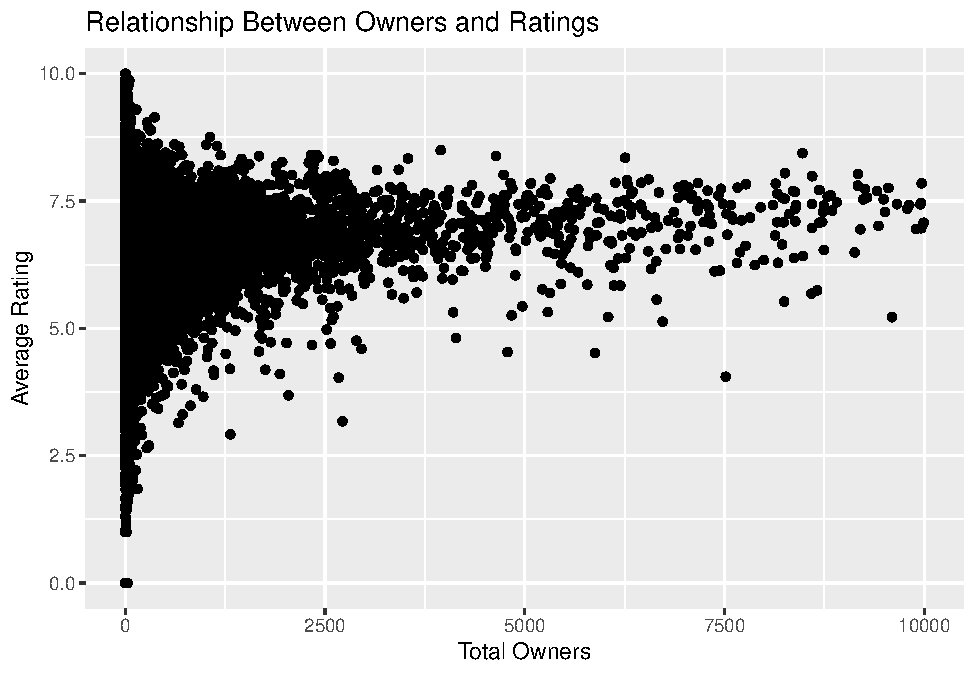
\includegraphics{AssI_CompStat2023_files/figure-latex/unnamed-chunk-3-1.pdf}

\begin{Shaded}
\begin{Highlighting}[]
\FunctionTok{hist}\NormalTok{(y1,}\AttributeTok{breaks =} \DecValTok{30}\NormalTok{, }\AttributeTok{freq=}\NormalTok{F)}
\end{Highlighting}
\end{Shaded}

\includegraphics{AssI_CompStat2023_files/figure-latex/unnamed-chunk-3-2.pdf}

\hypertarget{exercise-4}{%
\section{Exercise 4}\label{exercise-4}}

\hypertarget{point-a-2}{%
\subsection{Point a}\label{point-a-2}}

We write the probability of a standard Normal r.v. X as an integral
thanks to its probability density function.

\(P(X>20)=\int_{20}^\infty \frac{1}{\sqrt{2\pi}} e^{-\frac{x^{2}}{2}} dx\)

Reference: Wikipedia

The crude Monte Carlo estimation of this quantity is deemed to fail
because the region of integration is so far out in the tails of the
standard normal distribution.

\hypertarget{point-b}{%
\subsection{Point b}\label{point-b}}

Rewrite the integral employing the change of variable
\(Y = \frac{1}{X}\).

\(dy=-\frac{1}{x^{2}} dx\\dx=-x^{2}dy=-\frac{1}{y^{2}}dy\\y=Y_{20}=0,05\\y=Y_\infty=0\)

So
\(\int_{20}^\infty \frac{1}{\sqrt{2\pi}} e^{-\frac{x^{2}}{2}} dx\\=\int_{0,05}^0 \frac{1}{\sqrt{2\pi}} e^{-\frac{1}{2y^{2}}} -\frac{1}{y^2} dy \\=\int_0^{0,05} \frac{1}{\sqrt{2\pi}} e^{-\frac{1}{2y^{2}}} \frac{1}{y^2} dy\)

\end{document}
